%%%%%%%%%%%%%%%%%%%%%%%%%%%%%%%%%%%%%%%%%%%%%%
\section{Beam requirements}
\label{sec:beamrequirements}

The requested beam parameters are driven by the requirement that the results from the CERN test beam should be directly applicable to the future large underground single-phase LAr detector with minimal extrapolation. The CERN test beam data will be used to evaluate the detector performance, to understand the various physics systematic effects, and to provide data for event reconstruction studies that are representative of neutrino interactions. To satisfy the requirement, the beam parameters must span a broad range of particle momenta to match the charged particle spectrum and topologies that are expected in the DUNE far detector. The particle beam composition should consist of electrons, muons, and hadron and need to be charge-selected. The expected momentum distributions for secondary particles from neutrino interactions are shown in Figure~\ref{fig:ParticleMomenta}. There is a large spread in the momentum distribution with most particles peaked near 200 MeV/c.  
The desirable momentum range for ProtoDUNE-SP  is in the low momentum region. Based on the feedback and constraints from the CERN beam group, the requested beamline design allows the transport of beam particles from about 0.2 GeV/c up to 7 GeV/c. 
\fixme{also need to address particle interaction topologies; should use consistently 0.5 GeV as lower limit}

The maximum electron drift time in the TPC is about 2.25 ms. In order
to keep the  pile-up in the TPC at the percent-level, the planned
beam rate should not exceed 100 Hz.  
The ProtoDUNE-SP TPC has two drift volumes separated by a
passive cathode plane. It is desirable to aim the particle beam such
that a large fraction of the lower energy hadronic showers are mostly
contained in one drift volume, thus minimizing the uncertainties from
particles lost in the inactive detector materials. It is also
important to be able to inject beam into the cryostat at multiple
locations to study the detector
response. Figure~\ref{fig:beamwindow_loc} shows the three proposed
beam injection points.  The angles of the beam, w.r.t. the APA plane
are 3$^\circ$ (beam \#1), 8$^\circ$ (beam \#2), and 12$^\circ$ (beam
\#3). Due to engineering and safety considerations, only beam \#3 will
be fully instrumented with the beam window system as described in
Sections~\ref{subsec:beamwindow} and~\ref{sec:beamplug}. The remaining two beam positions will have
partial installation of the beam window system. With this
configuration, beam \#3 is the primary beam where most of the physics
data will be taken.
\begin{cdrfigure}[Beam window locations]{beamwindow_loc}{Planned beam window locations.}
  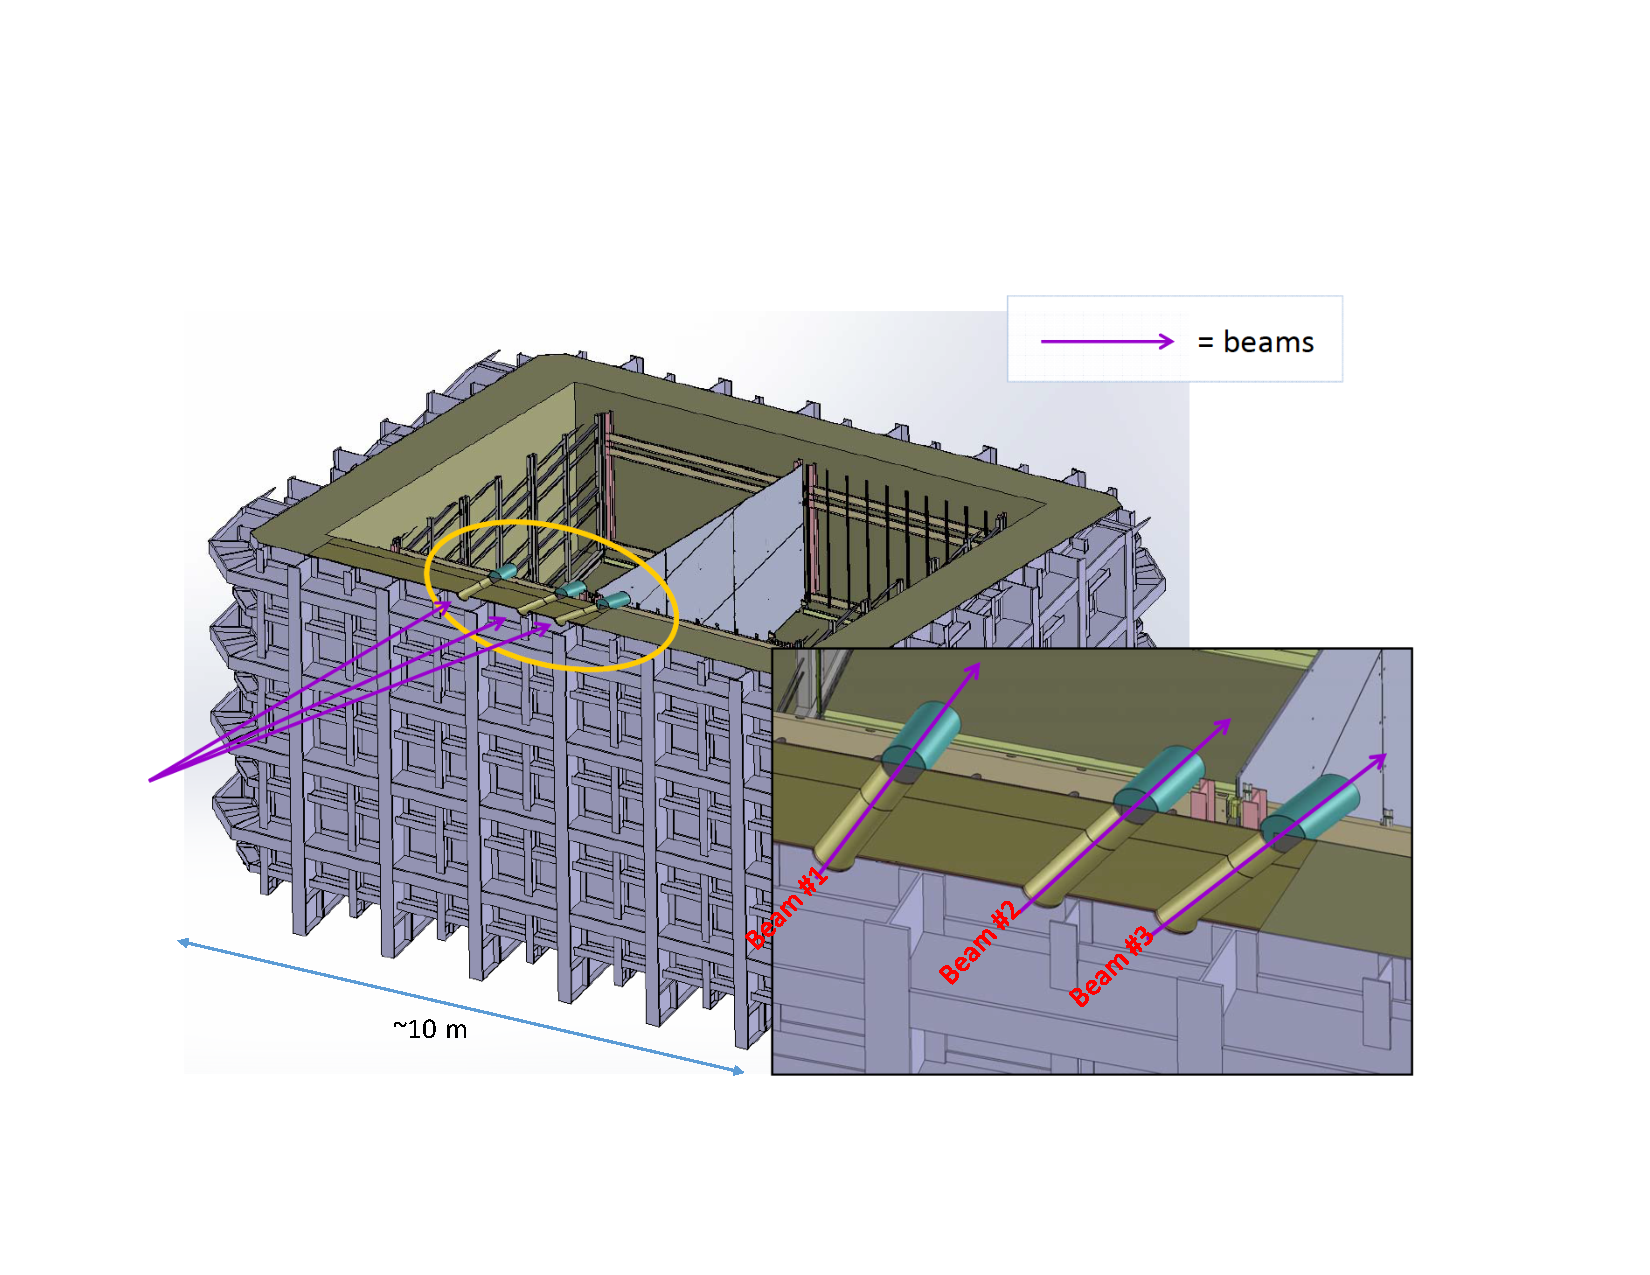
\includegraphics[width=0.9\textwidth]{beamwindow_locations.pdf}
\end{cdrfigure}
The summary of the beam requirements are shown in Table~\ref{tab:beamspecs}.
\begin{cdrtable}[Particle beam requirement]{cc}{beamspecs}{Particle beam requirements}
%\textbf{Parameter } & \textbf{Requirements}  \\ \hline
 Parameter & Requirements \\ \toprowrule
  Particle Types        & $e^\pm,\mu^\pm,\pi^\pm$,$K$,$p$  \\ \colhline
  Momentum Range   & 0.2 - 7 GeV/$c$ \\ \colhline
  Momentum Spread   & $\Delta p/p  < $5 \% \\
  & (limited by the aperture of the magnets)  \\ \colhline
  Transverse Beam Size   & RMS(x,y) $\approx$ 1 cm  \\
  & (At the entrance face of the LAr cryostat) \\ \colhline
  Beam Divergence & tbd   \\ \colhline
  Beam Entrance Position & Multiple beam windows    \\ \colhline
  Rates & 100 Hz (maximum)    \\ \colhline
\end{cdrtable}

\fixme{put K in parentheses and provide appropriate moment in caption; lower momentum range should be 0.5 GeV (see CERN workshop discussion) }
\fixme{momentum spread/characterization: need tomato clear that this is w/o any beam monitor information}
\fixme{we should have beam divergence estimates from H2 and H4 simulation files}
\fixme{rate: max of 100 Hx; nominal 25Hz with goal to achieve 50 Hz (see CERN workshop)}
